% SHEAF Gate 0 vs Agrimate (Kuhla, Kubiczek & Otto, Ecological Economics 231, 2025)
% Overleaf: New Project → Upload Project → zip this folder (main.tex + figures/ + tables/).
\documentclass[11pt,a4paper]{article}
\usepackage[margin=1in]{geometry}
\usepackage{graphicx}
\usepackage{booktabs}
\usepackage{tabularx}
\usepackage{amsmath}
\usepackage{siunitx}
\usepackage{xcolor}
\usepackage{hyperref}
\usepackage{caption}
\usepackage{subcaption}
\usepackage{float}

\hypersetup{colorlinks=true,linkcolor=black,citecolor=black,urlcolor=blue}
\graphicspath{{figures/}}

\title{SHEAF Gate 0 against Agrimate's per-commodity hindcast\\
\large Wheat, maize, and rice, 2006--2011}
\author{SHEAF working note (not a journal submission)}
\date{\today}

\begin{document}
\maketitle

\begin{abstract}
Agrimate (Kuhla et al., 2025) is a single-commodity, 24-step-per-year agent-based
trade model. Its published validation is (i)~wheat world prices and annual
supply/stock changes in the main text (Figs.~3--4), (ii)~a Russia--Egypt
mechanism case (Figs.~5--7), and (iii)~the same price split for rice, maize, and
soybean in Supplement~G. SHEAF's Gate~0 spine is the same clock and the same
forcing (USDA PSD harvests + AMIS quantity cuts), one crop at a time, with
cross-grain substitution and the endogenous export game switched off.
This note reruns Agrimate's \emph{scenario split} on SHEAF and reports, without
cosmetics, where the checks match and where they do not.
The full Gate~0 writeup (mathematics, parameterization, 2021--23 Ukraine-war
hindcast, leftovers) is \texttt{overleaf/gate0\_whitepaper/}; do not treat this
folder as the paper.
\end{abstract}

\section{What Agrimate actually checked}

Agrimate does \emph{not} publish a multi-commodity model. Wheat is the main-text
bar; rice, maize, and soybean are calibrated separately and shown only as
harvest / restricted-exports / world-price panels (Suppl.\ Figs.~G.1--G.3).
The scenarios are always:
\begin{enumerate}
  \item \textbf{baseline} --- climatology harvest, no export restrictions;
  \item \textbf{production anomalies} --- year-by-year harvest, no restrictions;
  \item \textbf{full} --- harvest anomalies plus historical AMIS restrictions.
\end{enumerate}
World price is the export-volume-weighted offer price, compared to a US-CPI
deflated Pink Sheet series. Annual supply and stock \emph{changes} are compared
to FAOSTAT as percent of 2007--2009 mean supply. Regional maps are wheat, 2007
only.

SHEAF Gate~0 uses the same three legs as Agrimate. Official P1 \textbf{matched}
is harvest + AMIS + mean flex (USA maize industrial on). A fourth \textbf{SHEAF}
leg also forces year-by-year PSD food/feed; Agrimate's published full run does
not, so that extra leg is a sensitivity (purple dashed in the price panels).

Soybean is out of SHEAF's grain set. The 2022 Ukraine wheat exercise
(Agrimate Suppl.\ Fig.~A.5) is not in this figure factory; it is scored in
the white paper (\texttt{scripts/score\_ukraine\_war.py}).

\section{Check-by-check status}

\begin{table}[H]
\centering
\caption{Agrimate published checks vs SHEAF Gate~0. ``Matched'' means the same
\emph{object} is computed, not that the numbers agree.}
\small
\begin{tabularx}{\textwidth}{l l X}
\toprule
Agrimate object & In SHEAF? & Notes \\
\midrule
24 steps/year clock & yes & locked \\
LOWESS harvest anomalies, USDA PSD & yes & \\
AMIS bans $\approx 95\%$, taxes $\approx 50\%$ quantity cuts & yes & \\
Fig.~3 harvest, anomaly, restricted MMT & yes & Fig.~\ref{fig:force-wheat} \\
Fig.~4a three-scenario world price vs Pink Sheet & yes & Fig.~\ref{fig:px-wheat} \\
Fig.~4b,e global annual supply/stock \emph{changes} & partial & PSD not FAOSTAT; marketing-year end \\
Fig.~4c--g 2007 regional maps (28 regions) & partial & 17 nodes + RoW, bar charts \\
Figs.~5--7 Russia supplier / Egypt / bilateral share & yes & Figs.~\ref{fig:ru}--\ref{fig:eg} \\
Suppl.\ G rice and maize price split & yes & Figs.~\ref{fig:px-rice},\ref{fig:px-maize} \\
Soybean G.3 & no & not a SHEAF grain \\
Suppl.\ F parameter sensitivity & no & not in this note \\
Nash-baseline \emph{seasonal} unperturbed price & no & SHEAF baseline is flat at $p_0$ (twin identity) \\
Cross-commodity substitution & off & blocked until Gate~0 is accepted \\
Endogenous export game & off & Level~2, later \\
\bottomrule
\end{tabularx}
\end{table}

The last two rows are design, not failures. The seasonal-baseline gap is real:
Agrimate's unperturbed run still wiggles with harvest and storage cost; SHEAF's
twin is an identity ($p^\star=p_0$ when free stocks, unmet, and blockage match
the twin). That is why the grey baseline in our price panels is nearly a
horizontal line.

\section{Wheat (Agrimate main text)}

\subsection{Forcing (their Fig.~3)}

\begin{figure}[H]
\centering
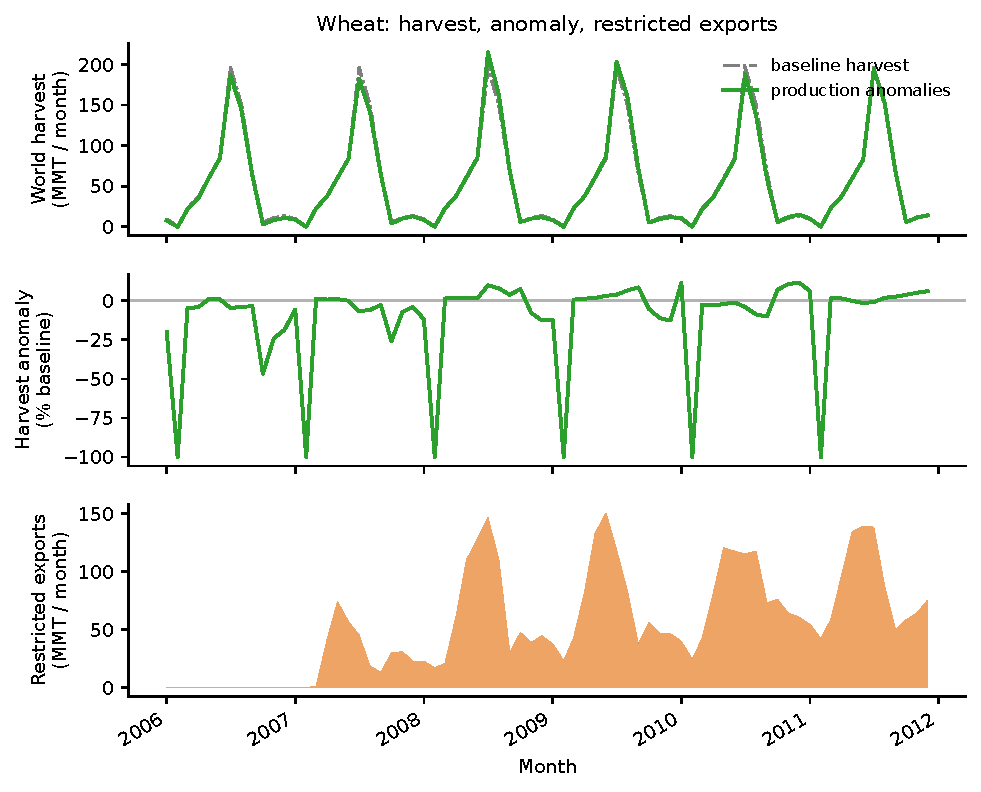
\includegraphics[width=\textwidth]{fig_forcing_wheat}
\caption{Wheat harvest (climatology vs realized), harvest anomaly, and AMIS-implied
restricted export volume. Restricted volume is
$O_{i,t}\,\tau_{i,t}/(1-\tau_{i,t})$ from the matched full run --- grain that would
have been offered without the cut. Compare Kuhla et al.\ Fig.~3.}
\label{fig:force-wheat}
\end{figure}

\subsection{World price (their Fig.~4a)}

\begin{figure}[H]
\centering
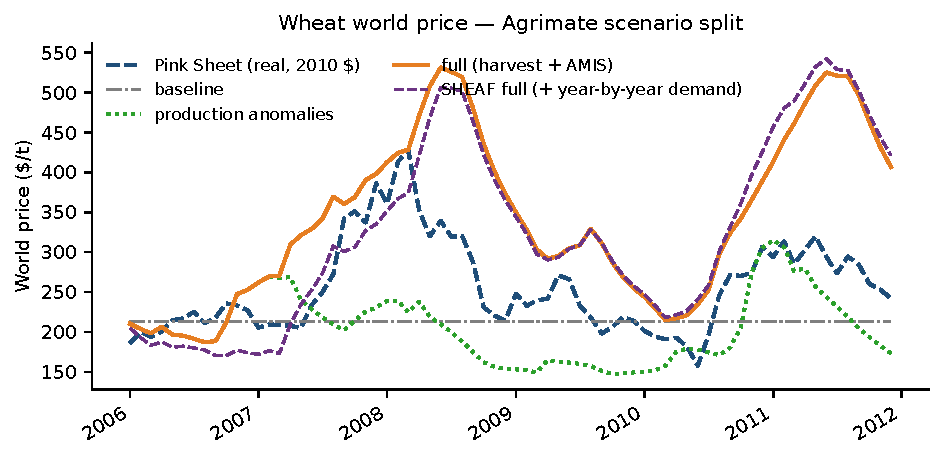
\includegraphics[width=\textwidth]{fig_prices_wheat}
\caption{Wheat world price under Agrimate's three scenarios, plus Pink Sheet
(US HRW, real). The purple dashed line is SHEAF full with year-by-year PSD demand;
Agrimate's published full run does not force that series.}
\label{fig:px-wheat}
\end{figure}

% auto-generated by scripts/make_agrimate_comparison.py
\begin{tabular}{l rr rrr rrr}
\toprule
 & \multicolumn{3}{c}{monthly corr} & \multicolumn{3}{c}{2007/08 hike} & \multicolumn{3}{c}{2010/11 hike} \\
\cmidrule(lr){2-3}\cmidrule(lr){4-6}\cmidrule(lr){7-9}
Crop & matched & SHEAF & matched & SHEAF & obs & matched & SHEAF & obs \\
\midrule
wheat & +0.72 & +0.62 & $\times$2.27 & $\times$2.14 & $\times$1.82 & $\times$1.45 & $\times$1.57 & $\times$1.16 \\
maize & +0.71 & +0.74 & $\times$1.97 & $\times$2.04 & $\times$1.84 & $\times$1.70 & $\times$1.77 & $\times$1.44 \\
rice & +0.68 & +0.70 & $\times$1.72 & $\times$1.97 & $\times$1.84 & $\times$0.82 & $\times$0.85 & $\times$0.79 \\
\bottomrule
\end{tabular}


The 2007/08 hike is the hard Agrimate bar (signs and timing). Isolated production
anomalies do not carry that hike on their own --- restrictions do
($\tau\times 1.70$ vs harvest $\times 1.20$; matched full $\times 2.27$ vs obs
$\times 1.82$). That matches Agrimate's \emph{2010} restriction language more
than their 2007 ``production-led'' reading; we do not relabel 2008 to match them.
After LOWESS detrend, 2010 wheat is production-led (harvest $\times 1.85$ vs
$\tau\times 1.36$). Pink Sheet here is MUV 2010\$; Agrimate Fig.~4a is CPI ---
compare ratios, not dollar levels.

\subsection{Global supply and stocks (their Fig.~4b,e)}

\begin{figure}[H]
\centering
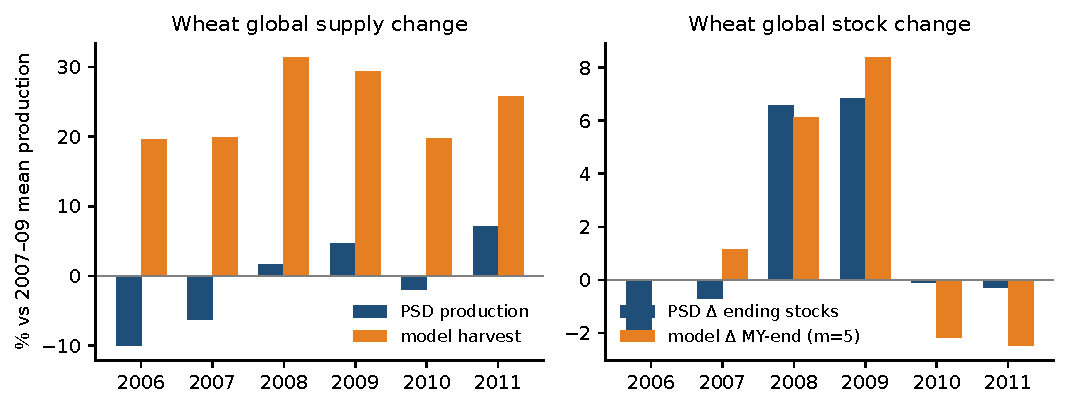
\includegraphics[width=\textwidth]{fig_balance_wheat}
\caption{Annual wheat supply change (production vs 2007--09 mean) and stock
change (year-to-year, as percent of mean production). Observed series is USDA PSD,
not FAOSTAT. Model stocks are marketing-year end (May), which is the comparable
month to PSD wheat ending stocks. Compare Kuhla et al.\ Fig.~4b,e.}
\label{fig:bal-wheat}
\end{figure}

% auto-generated
\begin{tabular}{l cc}
\toprule
Crop & Supply-change sign (6 y) & Stock-change sign (5 y) \\
\midrule
wheat & 3/6 & 4/5 \\
maize & 3/6 & 5/5 \\
rice & 3/6 & 3/5 \\
\bottomrule
\end{tabular}


\subsection{Regional 2007 (their Fig.~4c--g)}

\begin{figure}[H]
\centering
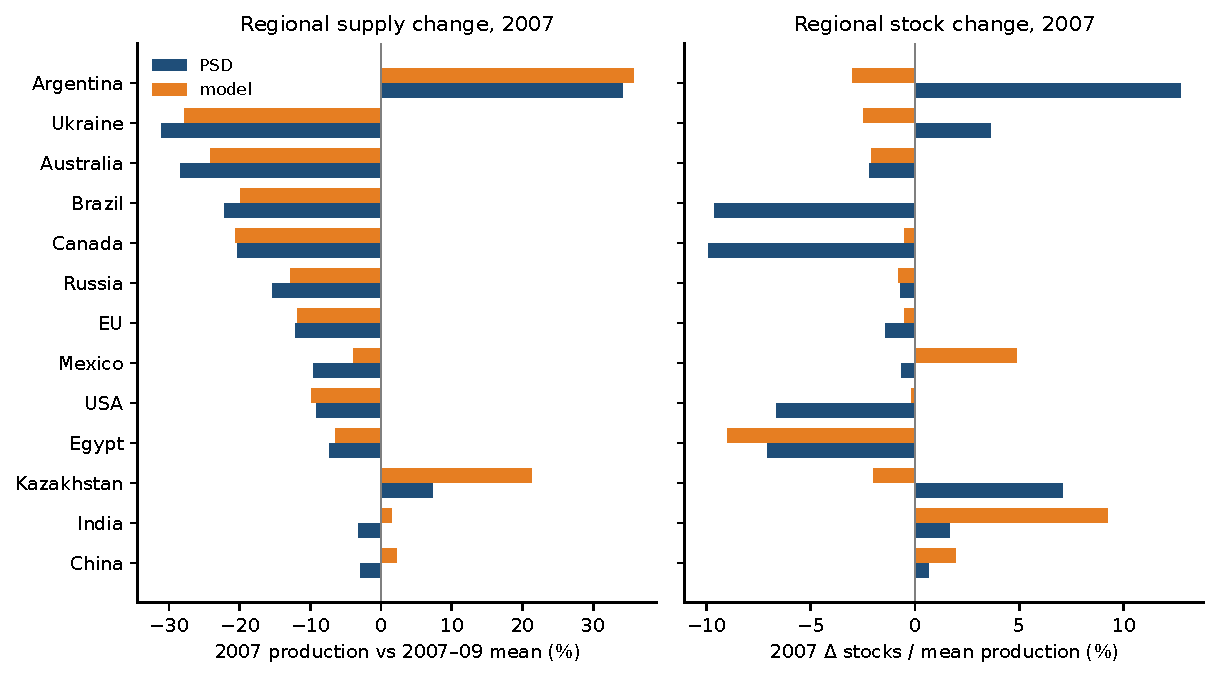
\includegraphics[width=\textwidth]{fig_regional2007_wheat}
\caption{2007 regional production and stock-change anomalies, SHEAF nodes vs PSD.
Agrimate maps 28 regions against FAOSTAT; we cannot replicate that map from the
node set. Sign agreement at the node level is the check.}
\label{fig:reg-wheat}
\end{figure}

\subsection{Russia and Egypt (their Figs.~5--7)}

\begin{figure}[H]
\centering
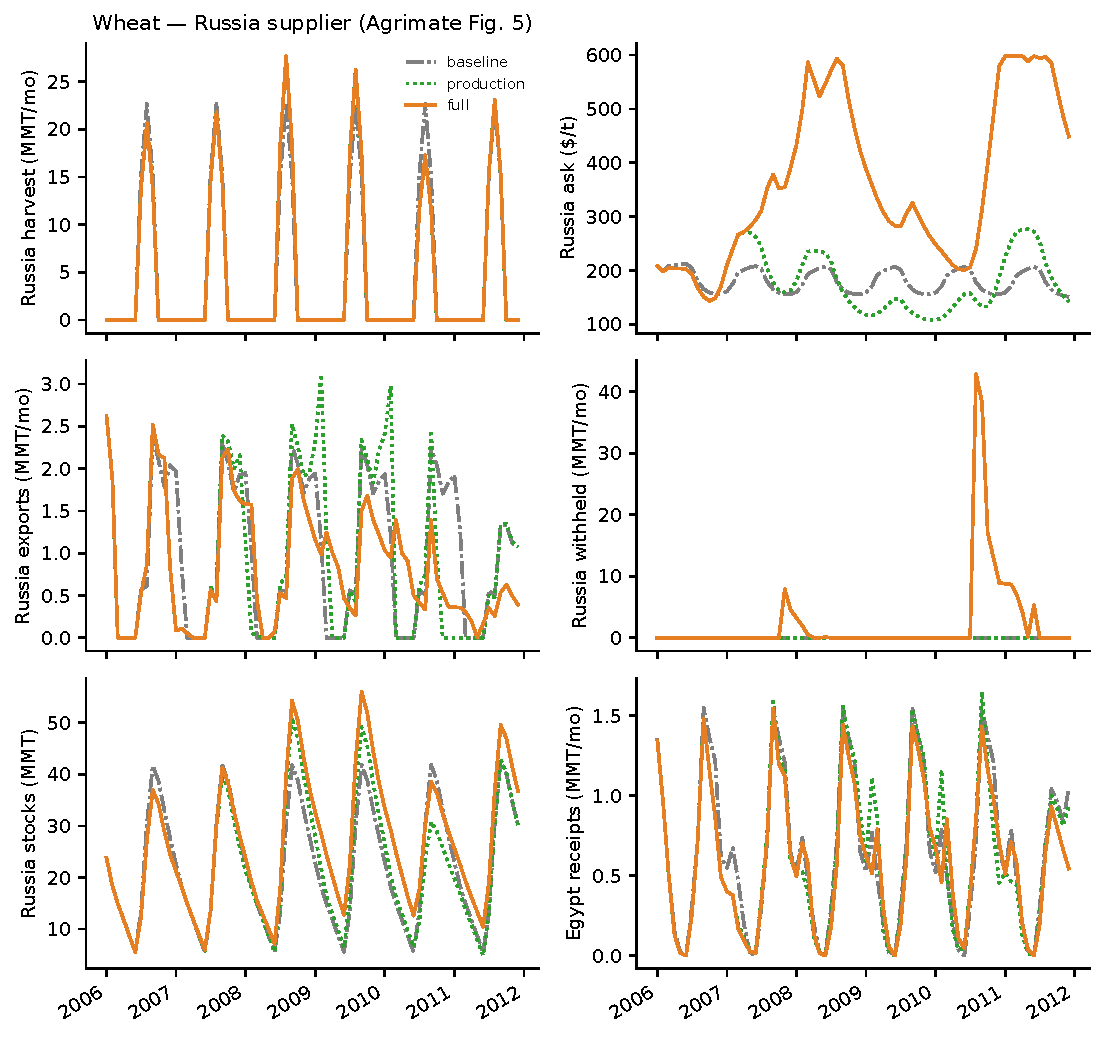
\includegraphics[width=\textwidth]{fig_russia_wheat}
\caption{Russia wheat: harvest, ask, exports, withheld volume, and stocks, plus
Egypt's receipts. SHEAF has one ask per exporter (no separate domestic vs
international offer). Compare Kuhla et al.\ Fig.~5.}
\label{fig:ru}
\end{figure}

\begin{figure}[H]
\centering
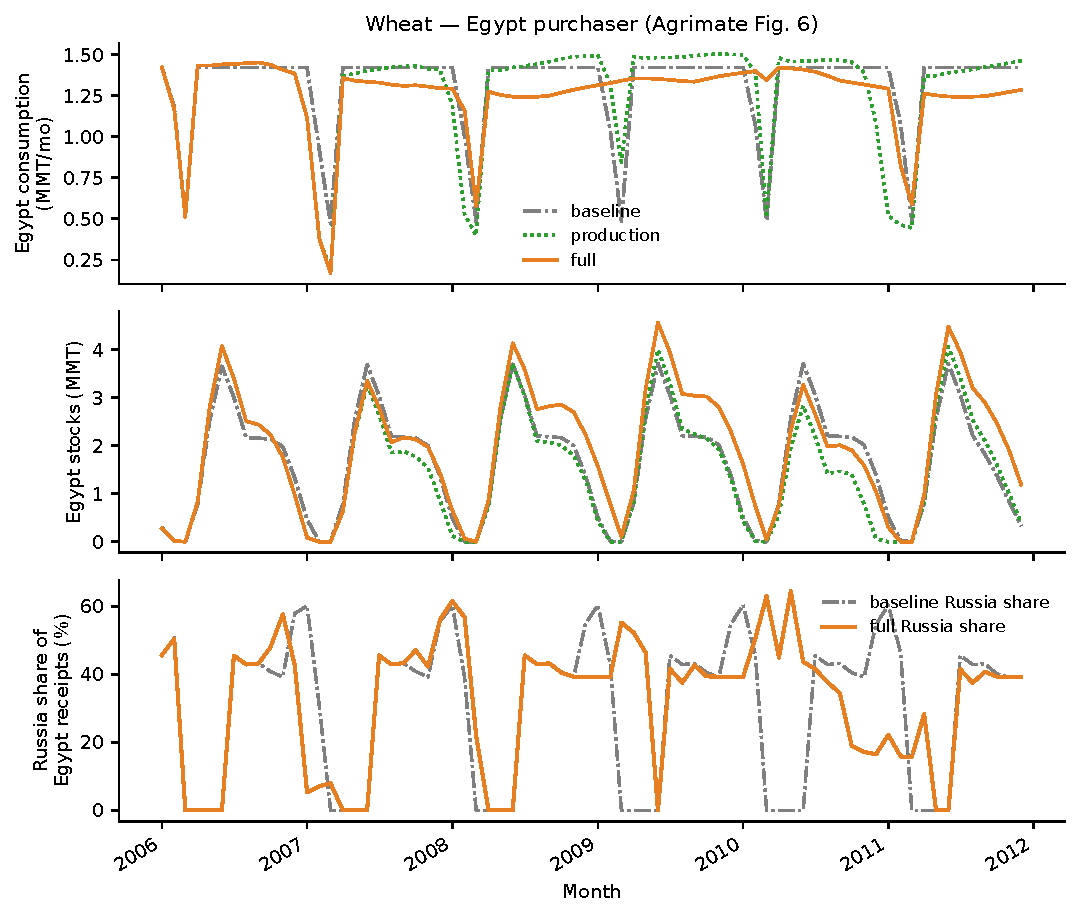
\includegraphics[width=\textwidth]{fig_egypt_wheat}
\caption{Egypt wheat consumption, stocks, and Russia's share of receipts.
Compare Kuhla et al.\ Figs.~6--7. Rerouting after the 2010 ban should cut that
share; if it does not, the Armington residual is too stiff.}
\label{fig:eg}
\end{figure}

\section{Rice and maize (Agrimate Supplement G)}

Agrimate's maize and rice bar is \emph{only} this three-panel split --- not the
regional maps. We run the same split.

\begin{figure}[H]
\centering
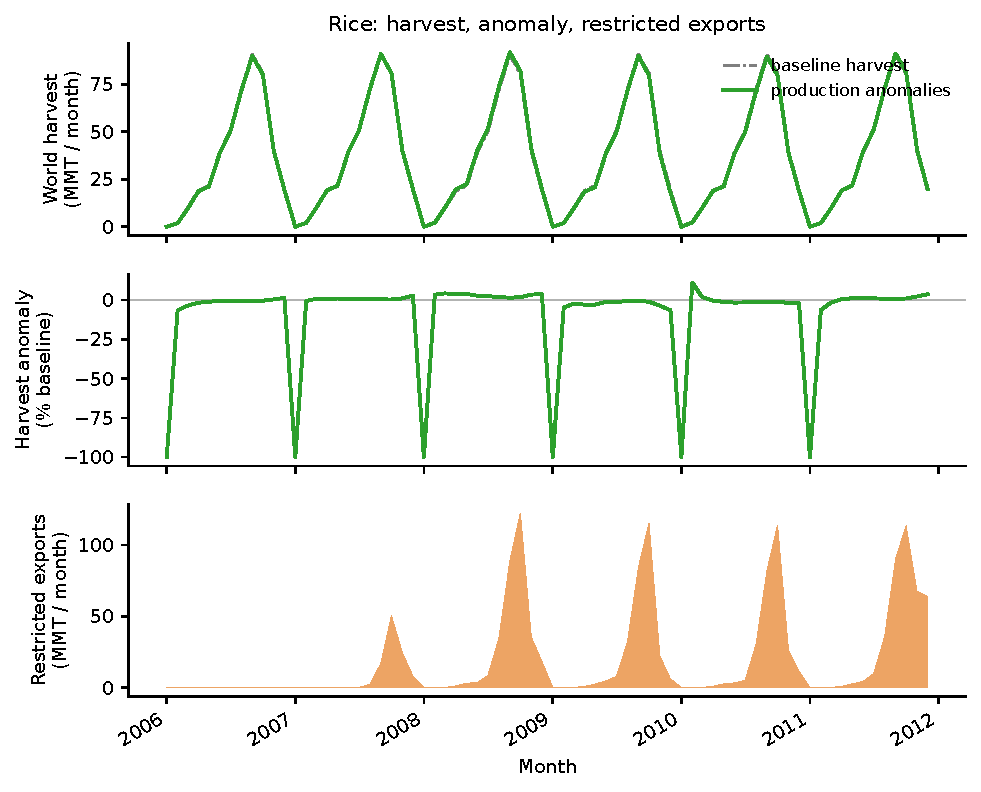
\includegraphics[width=\textwidth]{fig_forcing_rice}
\caption{Rice harvest, anomaly, and restricted exports. Agrimate: 2008 spike is
restriction-led on a better-than-usual harvest (Suppl.\ Fig.~G.1).}
\label{fig:force-rice}
\end{figure}

\begin{figure}[H]
\centering
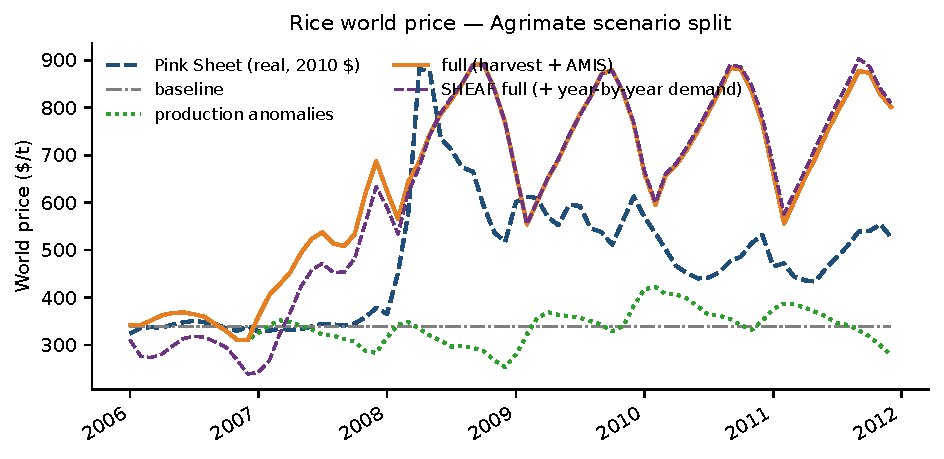
\includegraphics[width=\textwidth]{fig_prices_rice}
\caption{Rice world price, Agrimate scenario split vs Pink Sheet.
Compare Suppl.\ Fig.~G.1c.}
\label{fig:px-rice}
\end{figure}

\begin{figure}[H]
\centering
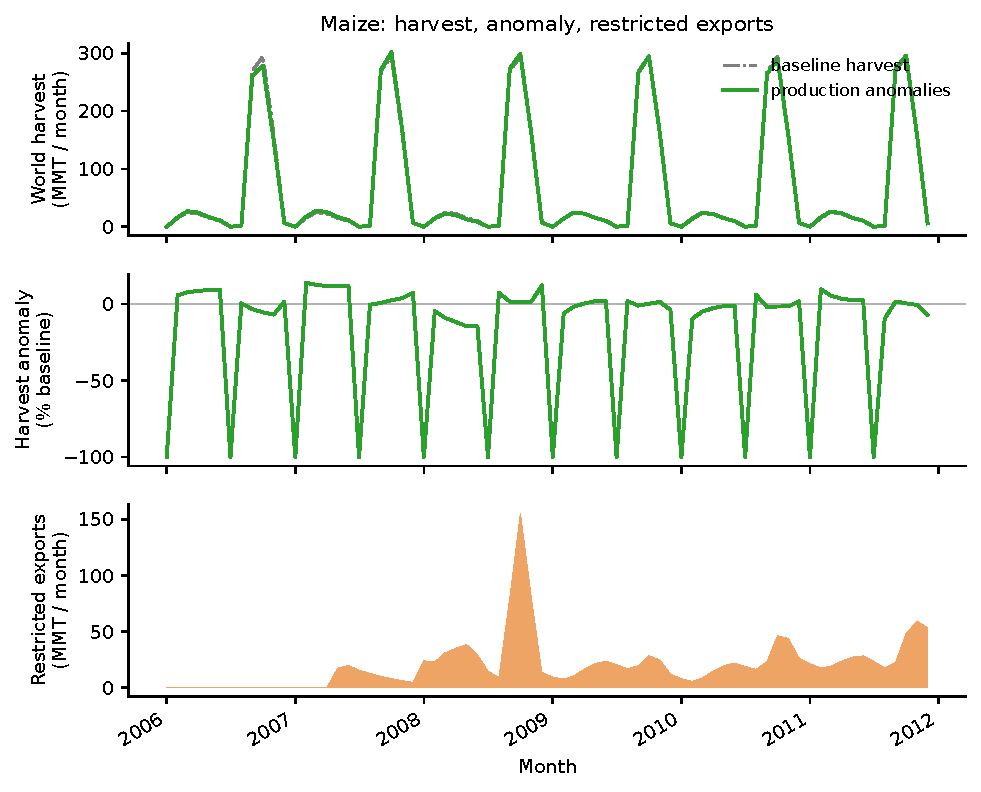
\includegraphics[width=\textwidth]{fig_forcing_maize}
\caption{Maize harvest, anomaly, and restricted exports. Agrimate: 2008 peak
restriction-led on a stable harvest; 2011 harvest-failure-led (Suppl.\ Fig.~G.2).}
\label{fig:force-maize}
\end{figure}

\begin{figure}[H]
\centering
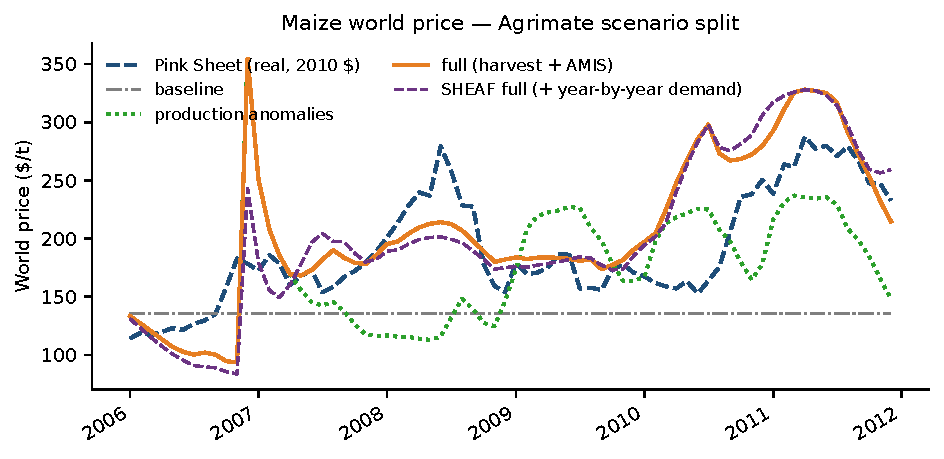
\includegraphics[width=\textwidth]{fig_prices_maize}
\caption{Maize world price, Agrimate scenario split vs Pink Sheet.
Purple dashed: SHEAF full with US industrial/ethanol (FSI excess vs 2000--04),
which Agrimate does not isolate. Compare Suppl.\ Fig.~G.2c.}
\label{fig:px-maize}
\end{figure}

\begin{figure}[H]
\centering
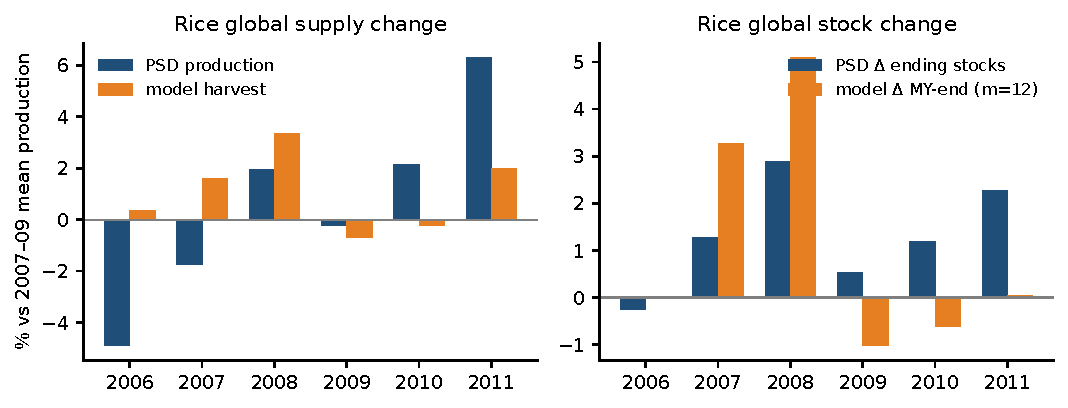
\includegraphics[width=0.95\textwidth]{fig_balance_rice}\\[0.6em]
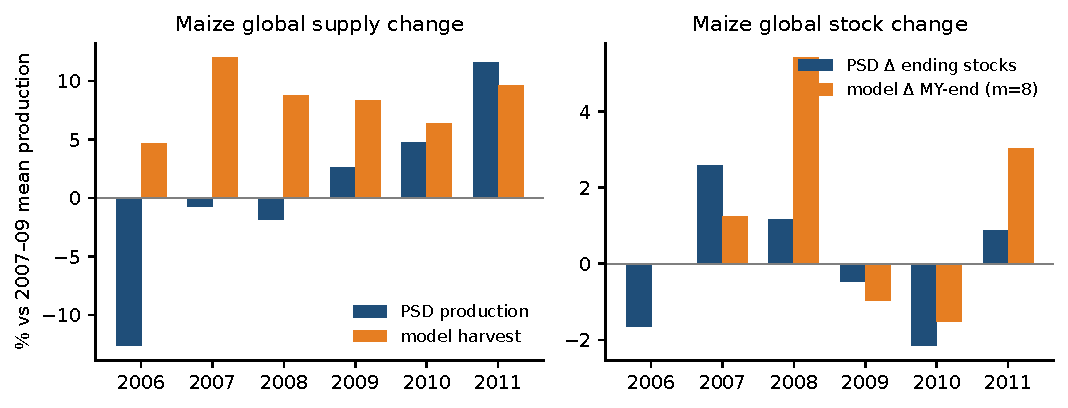
\includegraphics[width=0.95\textwidth]{fig_balance_maize}
\caption{Rice (top) and maize (bottom) global supply and stock-change signs.
Maize model stocks are August marketing-year end; December is post-harvest and
is the wrong comparison to PSD.}
\end{figure}

\section{Locked scores versus Agrimate (not a retune list)}

Official P1 is the matched column of the price-metrics table (harvest + AMIS, mean
flex, USA maize industrial on). Numbers: wheat corr $+0.72$, 2007/08
$\times 2.27$ vs $\times 1.82$, 2010/11 $\times 1.45$ vs $\times 1.16$;
maize $+0.71$, $\times 1.97$ vs $\times 1.84$, $\times 1.70$ vs $\times 1.44$;
rice $+0.68$, $\times 1.72$ vs $\times 1.84$, $\times 0.82$ vs $\times 0.79$.
Asserts PASS. Full narrative and leftovers:
\texttt{overleaf/gate0\_whitepaper/}.

\begin{itemize}
  \item \textbf{Wheat 2008} overshoots ($\times 2.27$ vs $\times 1.82$),
        restriction-led. 2006/07 residual tightness vs trend remains
        ($\times 1.46$ vs obs $\sim\times 0.95$). Not damped with a dummy.
  \item \textbf{Wheat 2010} is production-led after LOWESS. Agrimate's 2010
        restriction-led reading is a different harvest construction.
  \item \textbf{Maize 2008} matched is industrial-demand-led. Agrimate
        Suppl.\ Fig.~G.2 is restriction-led on a stable harvest. Isolated
        SHEAF $\tau$ must not cut the 14-month mean world price --- that
        assert stands. Different identification, disclosed.
  \item \textbf{Rice 2008} restriction-led on a non-crash harvest --- aligned
        with Suppl.\ Fig.~G.1. Year-by-year demand still worsens 2010; headline
        keeps mean flex.
  \item \textbf{Twin / baseline} is flat at $p_0$ (identity). Agrimate's
        unperturbed run still wiggles. Compare treatment deviations, not grey
        baselines.
  \item \textbf{Global stock-change signs} (table below Fig.~\ref{fig:bal-wheat})
        are mixed; world MY-end \emph{levels} vs PSD are on the bar
        (wheat $\times 1.02$, maize $\times 1.08$, rice $\times 1.05$).
  \item \textbf{Russia share of Egypt receipts} drops in 2010/11 under AMIS
        --- mechanism check passes.
  \item \textbf{Sensitivity (their Suppl.~F)} not reproduced.
\end{itemize}

\textbf{Verdict.} Same checks. Rice 2008 and wheat 2010/2022 attribution agree
in the white paper. Maize 2008 identification differs for a documented RFS
reason. Substitution is the next paper, not a patch for leftovers.

\section{Reproducing the figures}

\begin{verbatim}
python scripts/make_agrimate_comparison.py
\end{verbatim}
writes \texttt{overleaf/gate0\_agrimate/figures/*.pdf} and
\texttt{tables/*.tex}. This folder is the Agrimate figure companion.
Upload the white paper instead: zip \texttt{overleaf/gate0\_whitepaper/}.

\end{document}
